\chapter{Generative Adversarial Networks - Améliorations}


\section{Apprentissage par Mini-Batch}
\subsection{Principe}
L'apprentissage par Batch consiste à apprendre sur l'ensemble du batch d'apprentissage avant de mettre à jour chaque réseau, et de réitérer l'apprentissage à chaque itération sur l'ensemble du batch d'apprentissage.

On calcule successivement la rétropropagation pour chaque image, on somme l'erreur sur l'ensemble des images et on applique la mise à jour du réseau avec la somme des erreurs. On obtient donc une moyenne des directions de propagation afin d'effectuer la mise à jour.

Certaines bases d'apprentissage étant très grandes - soixante mille avec MNIST par exemple -, on va préférer à l'apprentissage par batch, l'apprentissage par Mini-batch. 
On sélectionne aléatoirement parmi la base d'apprentissage et de tests un nombre plus petit d'éléments.
\subsection{Implémentation}
\paragraph{Mise à jour des poids}
Afin de pouvoir effectuer la rétro-propagation uniquement à la fin de l'itération du minibatch, nous avons simplement 

\paragraph{Sets d'apprentissage et de tests. plus petits}
Dans le cas de MNIST, les chiffres du début de la bdd étant plus simple, nous avons afin d'obtenir de meilleurs résultats parfois effectué une sélection aléatoire sur uniquement une première partie des 60000 images d'apprentissage (cf argument \textit{labelTrainSize}) et des 10000 images de tests (cf argument \textit{labelTestSize}.

\subsection{Résultats}
Notre équipe a obtenu des résultats peu convaincants, et très différents des résultats du groupe Salamandre 
Globalement, l'apprentissage s'effectue légèrement plus rapidement pour un même nombre d'itérations, au prix d'une augmentation du temps de calcul par itération (proportionnel selon la taille des batch). Cette technique a donc été abandonnée.
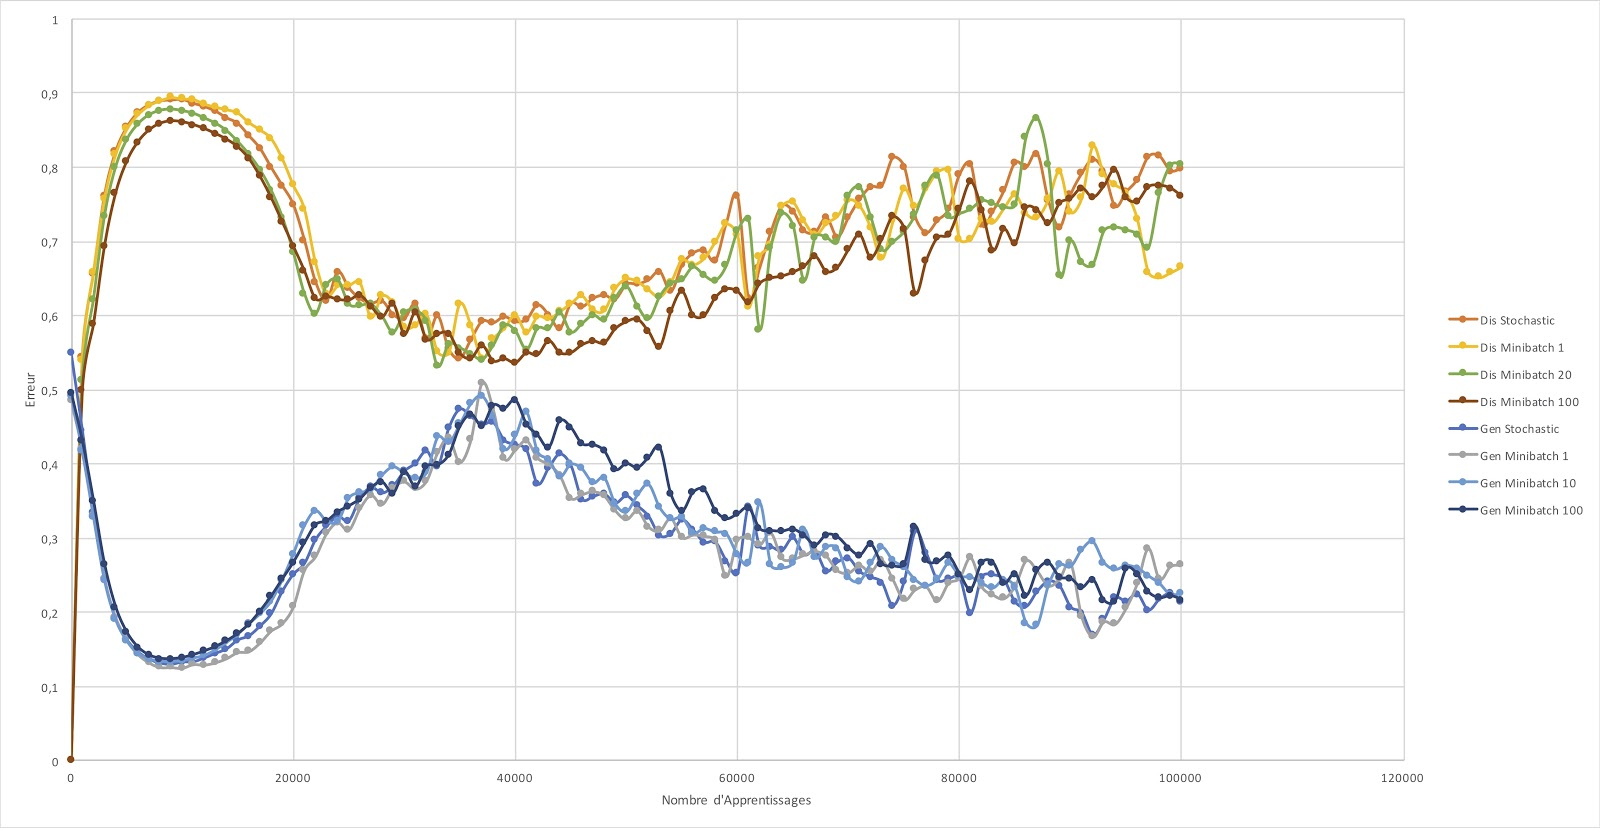
\includegraphics[width=1.5\textwidth]{images/08-gan_ameliorations_resultats_1.jpg}

\section{Algorithmes de pas d'apprentissage adaptatif}
\subsection{Principe}
L'objectif de ces algorithmes est de paramétrer au mieux la convergence de la distribution représentée par notre réseau vers la distribution $p_data$. Le pas adaptatif n'est alors plus constant; il varie en fonction du gradient des étapes d'apprentissage précédentes, de manière plus ou moins évoluée selon les algorithmes.

L'objectif est ainsi de faire évoluer le pas en fonction des erreurs, selon diverses formules. Deux méthodes de pas adaptatifs ont été utilisées : RMSprop et Adam. Nous en présentons ici d'autres.

\subsection{Adagrad}

Cette première méthode de descente adaptative suit les équations suivantes :

\begin{equation}
\begin{aligned}
g_{t+1} = g_t + (\frac{\partial J}{\partial W})^2 \\
W_{t+1} = W_t - \dfrac{\eta}{\sqrt{g_{t+1}} + \epsilon}\frac{\partial J}{\partial W}
\end{aligned}
\end{equation} 

Adagrad n'a pas été implémenté en raison des piètres performances annoncées\textsuperscript{[ref nécessaire])}. En effet, g est strictement croissante, étant incrémenté à chaque itération de $(\frac{\partial J}{\partial W})^2$ . Les réseaux apprenant sur un grand nombre d'itération, le coefficient $g_{t}$ devient rapidement très important, et le pas en $\dfrac{1}{\sqrt{g_{t+1}}}$ devient rapidement négligeable. Les performances de cet algorithme sont donc assez faibles.

\subsection{RMSprop}

La RMSProp permet de résoudre ce problème. En effet, on a un décroissance exponentielle de l'influence de l'erreur dans le temps grâce au coefficient $\gamma$ correspondant au moment d'ordre 2. Ainsi, l'influence des anciennes valeurs de $(\frac{\partial J}{\partial W})^2$ décroit exponentiellement, les erreurs les plus récentes sont donc les plus influentes sur le pas.

\begin{equation} 
\begin{aligned}
g_{t+1} = \gamma g_t + (1-\gamma)(\frac{\partial J}{\partial W})^2 \\
W_{t+1} = W_t - \dfrac{\eta}{\sqrt{g_{t+1}} + \epsilon}\frac{\partial J}{\partial W}
\end{aligned}
\end{equation} 

\subsection{Adam}

\begin{equation} 
\begin{aligned}
g_{t+1} = \gamma g_t + (1-\gamma)(\frac{\partial J}{\partial W})^2  \\
\hat{g}_{t} = \frac{g_{t} }{1 - \gamma^t} \\
m_{t+1} = \delta g_t + (1-\delta)\frac{\partial J}{\partial W}   \\
\hat{m}_{t} = \frac{m_{t} }{1 - \delta^t} \\
W_{t+1} = W_t - \dfrac{\eta}{\sqrt{\hat{g}_{t+1}} + \epsilon}\hat{m}_{t}
\end{aligned}
\end{equation} 

La méthode de descente de gradient AdamProp comprend deux aspects importants : le moment d'ordre 2 est conservé par rapport à la RMSProp, on a donc de nouveau cette décroissance exponentielle de l'influence des anciennes erreurs, qui vont pondérer le pas. De plus, elle prend en compte directement les anciennes valeurs de l'erreur, en remplaçant le terme d'erreur $\frac{\partial J}{\partial W}$ par $m_{t}$ qui correspond à un moment d'ordre 1 (moyenne). On garde donc en mémoire la tendance récente de l'erreur, ce qui permet d'adapter de façon plus précise le pas.
$\hat{g}_{t}$ et $\hat{m}_{t}$ sont des estimateurs corrigeant des  biais si les pas sont trop faibles.
Adam est considéré comme plus performante que RMSProp. 

\subsection{Utilisation}

La plupart de nos réseaux semblaient présenter une faiblesse au niveau du générateur, dont le score était trop souvent très faible, par rapport à un discriminateur très performant. Une meilleure descente pourrait donc accélérer et rééquilibrer ces apprentissages. 

Utiliser la RMSProp sur les deux réseaux permet d'apprendre des chiffres de belle qualité très rapidement (convergence jusqu'à 10 fois plus rapide que sous une descente de gradient normale), cependant on observe toujours ce déséquilibre entre les deux compétiteurs. Ce système semblait étrangement relativement instable, les paramètres amenant à la convergence étant assez restreints.

L’utilisation d’Adam pour le générateur et de RMSProp pour le discriminateur (ayant comme but d'entraîner mieux le générateur) semble bien fonctionner. La qualité des images est plus variable (le générateur produit des images laides et belles).
En revanche, l'utilisation de RMSProp pour le générateur et d'Adam pour le discriminateur ne fonctionne pas. Cela corrobore les résultats présentés par d'autres \cite{auriau_apprentissage_2017}[ref nécessaire : autre ref].

Enfin, si cela nous permet d'avoir un apprentissage plus performant, avec des images relativement belles en permettant au générateur de rester dans la course, cette solution ne permet pas de traiter le mode collapse : au contraire, l'apprentissage étant plus précis et rapide, on tombe très rapidement dans des états de mode collapse.

Ces apprentissages plus performants sont importants dans le sens où ils permettent un apprentissage plus performant des réseaux : celui-ci devrait être alors à la fois plus profond et plus précis. Cela permettrait alors de travailler correctement avec des réseaux plus grands, et des bases de données plus complexes avec des couches convolutives (CIFAR...).

\section{Réseaux de convolution}

\subsection{Implémentation}
Comme indiqué au \ref{implementation-C++-convolution}, nous avons dû coder la convolution à la main.
Afin de mettre en place un réseau à convolution, nous avons implémenté les différentes couches nécessaires : couche à convolution, couche de \textit{zero-padding} et couche de \textit{max-pooling}.
Néanmoins, l'implémentation en C++ du GAN à convolution ne s'est jamais comportée comme souhaitée. En effet, quel que soit le paramétrage, le réseau produit des résultats comparables à ceux obtenus avec un perceptron simple. Cela a donc eu des répercussions sur nos avancées (voir \ref{CIFAR-remarque-convolution})
Certaines fuites de mémoires ont été présentes par moment, mais uniquement sur une ou deux des quatre machines.

\subsection{Résultats}
Un réseau de configuration $784 \times 625 \times 100 \times 10$ avec uniquement une couche à convolution donne une erreur de 10\% comme classificateur de MNIST. [Manu : développer résultats du 25 mai (voir EdL et slides)]

\section{Échanges avec Giuseppe Valenzise}
Dans le domaine d'évaluation de la qualité des images, on distingue l'estimation avec référence (comparaison par rapport à une image) de l'estimation sans référence.
Maître de conférences au laboratoire L2S de CentraleSupélec, Giuseppe Valenzise est spécialiste en évaluation de qualité d'image (\textit{Visual Quality Assessment}) sans référence.
Les conclusions auxquelles nous avons pu aboutir au cours de l'échange étaient les mêmes que celles que nous avions pu formuler par le passé. Cela a néanmoins permis de les clarifier, et de nous confirmer l'intérêt du Wasserstein GAN. 
\begin{itemize}
\item L'évaluation d'une qualité d'image standard passe très souvent par l'usage de métriques (i.e. fonctions) appliquées sur les valeurs des pixels. Une métrique souvent proposée est NIQE (\textit{Naturalness Image Quality Evaluator}), qui consiste en la recherche de statistiques gaussiennes locales avec des coefficients mscn (\textit{mean subtracted and contrast normalized}). Néanmoins, les images utilisées dans notre étude (MNIST, CIFAR) sont beaucoup plus petites que des images standard (28x28 et 32x32 au lieu de plusieurs millions de pixels par image). L'estimation des gaussiennes est fortement bruitée, les métriques ne sont donc pas efficaces.
\item Les méthodes avancées d'évaluation de qualité d'image consistent en l'utilisation de classificateurs. On cherche à extraire des caractéristiques des images (vecteurs, symétries, ...) et on crée des classificateurs qui décident sur la base de ces caractéristiques. Le travail consiste alors à trouver les meilleures caractéristiques d'image.
\item Dans le cas des réseaux neuronaux, la distance entre les poids du réseau constitue une des caractéristiques les plus exploitées. G. Valenzise considère que dans le cas du GAN, la fonction de coût du discriminateur devrait constituer un des meilleurs classificateurs. Or dans le cas d'un GAN classique, nous avons pu remarquer qu'elle ne suit pas toujours la qualité des images.
\item Il nous a suggéré de réfléchir à un « réseau de classification » qui permettrait de s'affranchir de ces problèmes. Or, un tel réseau de classification existe déjà dans la littérature : Le WGAN.  
\item Le WGAN permet d'obtenir un meilleur lien entre qualité d'image et fonction de coût du discriminateur, le classificateur \textit{fonction de coût du réseau discriminant} est amélioré, en modifiant profondément sa structure.
\end{itemize}

\section{Pistes de recherche}
Cette section regroupe les pistes de recherche que nous avons pu rencontrer mais qui n'ont pas été approfondie faute de temps. Certaines pistes de recherches ne bénéficient pas de papiers à leur sujet.
\begin{itemize}
\item Étudier l’impact du nombre d’images disponibles dans la base d’entraînement. A priori, s’il est petit, l’effet d’apprentissage « par cœur » peut apparaître. Proposé par la chef de l’équipe de TaO du LRI.
\end{itemize}









